\section{1. Designing and building a typical ET experiment in our field }
Eye-movements provide a fine grain measure of various levels of language processing.
\parencite[e.g.][]{Tanenhaus_Spivey-Knowlton_Eberhard_Sedivy_1995,Allopenna_1998}. The now classic visual world paradigm (VWP) involves a 2x2 design including a target, competitor(s), and distractor(s) with a variety of possible formats from pictures to words.

\begin{figure}[ht]
    \centering
    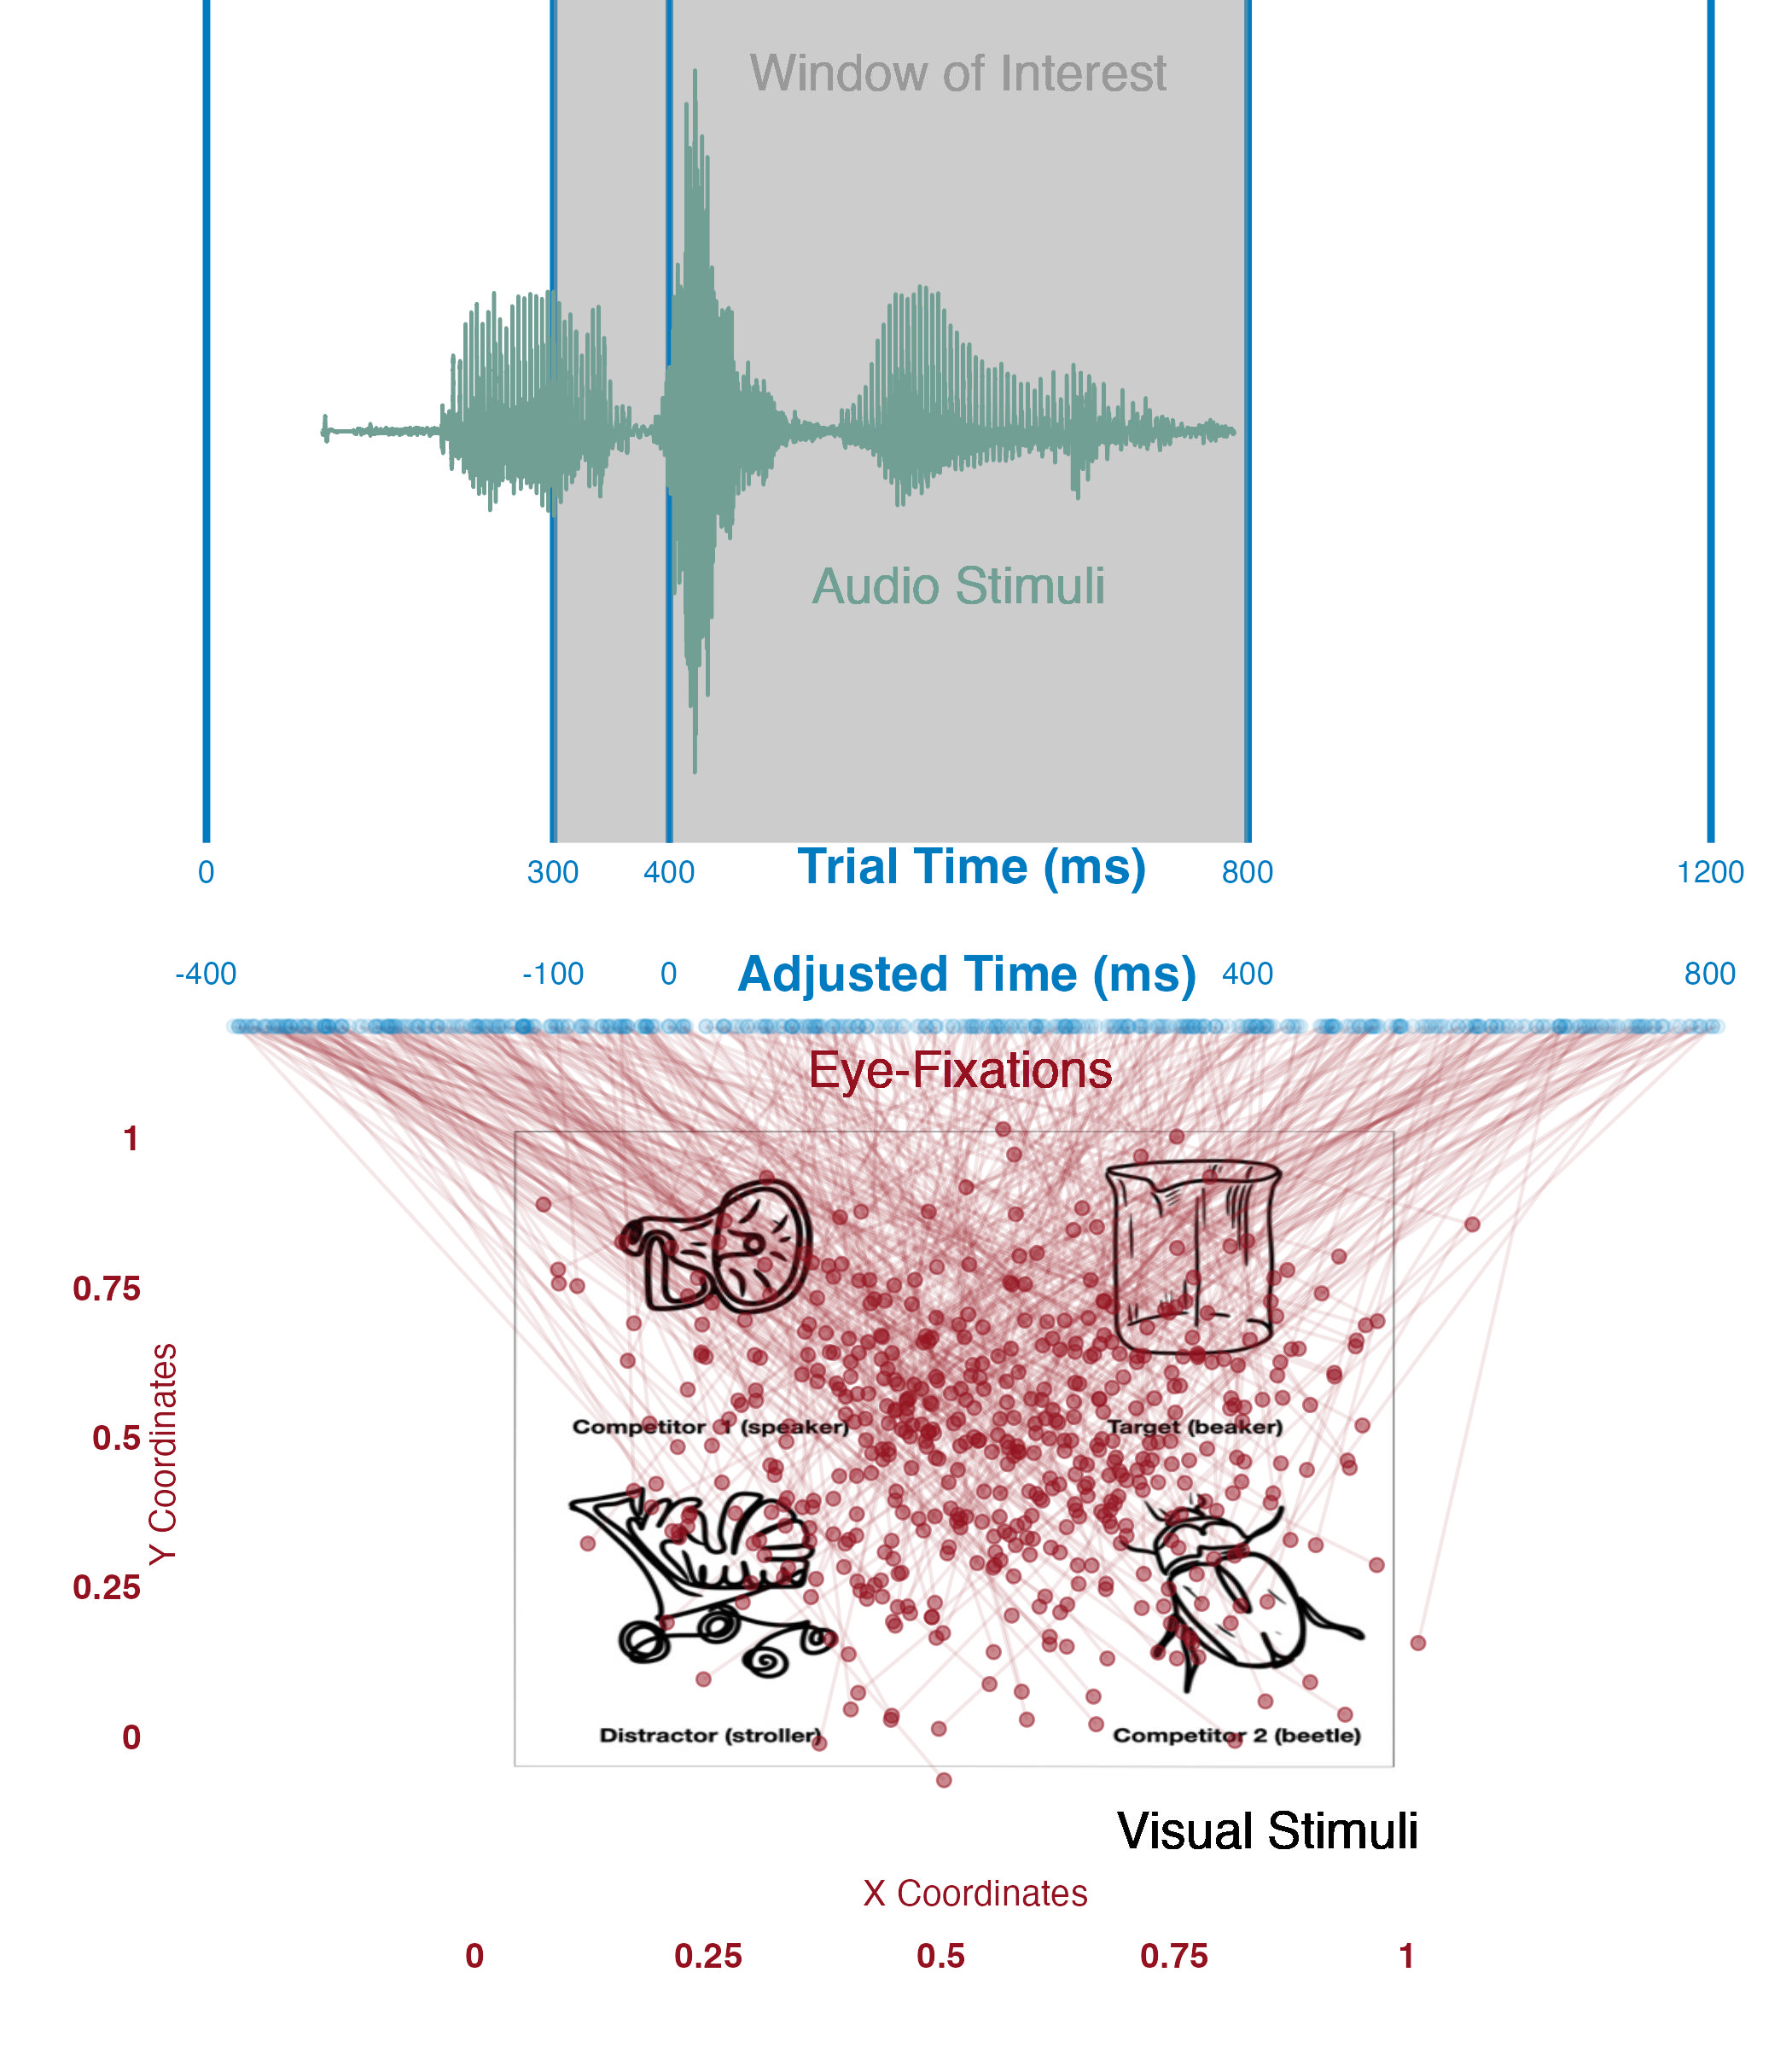
\includegraphics[height=.8\textwidth]{figures/Core_four_R.jpeg}
    \caption{A basic illustration of the core four constructs of the VWP. Eye fixations, represented by red dots, and respective times (blue dots) are a real sample from our data. Coloring is consistent throughout the paper for reference to four core constructs (i.e., time: blue, audio-stimuli: green, visual stimuli: black, eye-fixations: red). }
    \label{fig:core_four}
\end{figure}

As seen in figure \ref{fig:core_four}, for the VWP, a set of images are displayed on a screen time-locked to a point in an audio stimulus (e.g., beaker). Both previewing and delayed presentation of images is common. Ultimately, the specific timing used in a study depends on the design  \parencite[see,][, for a review]{Apfelbaum_Klein-Packard_McMurray_2021}{}{}.  The participant then either needs to select the correct answer based on the audio that they perceived or simply listen and look as the sound stimuli plays (e.g., passive listening). VWP experiments vary widely in what linguistic process is being investigated (e.g., referent prediction, sentence processing, word recognition, phonetic cue integration). However, all VWP experiments carefully control three core constructs (i.e., time, audio stimuli, and visual stimuli) in order to bring meaning to a fourth core construct: eye-fixations. 

For the remainder of this paper, these "core four" constructs will be used to guide the reader's understanding of how variation in eye-movement behavior can be captured, organized, and analyzed. 

\subsection{The core four of a 2x2 VWP experiment}

\textbf{Time.} Eye-tracking is especially valuable, in part, because it is an online measure that provides the time-course of processing. Time can be measured from the beginning of the trial to the end of the trial ('Trial Time' in figure \ref{fig:core_four}). There are two adjustments, however, that are often made to the time variable ('Adjusted Time'  in figure \ref{fig:core_four}). First, it typically takes a listener about 200 ms to plan an eye-movement \parencite[][]{Matin_Shao_Boff_1993}. Eye-movements within the first 200 ms are therefore discarded and researchers typically account for this 200 ms delay by adjusting the analysis. Second, within each trial there exists a window of interest (The greyed area in the top of figure \ref{fig:core_four}), which is only a portion of the full trial time corresponding to post-audio stimuli presentation. For example, time in which any carrier phrase is presented is typically ignored and time after the start of the target word is examined.

\textbf{Audio Stimuli.} This is the auditory input a participant receives on each trial. The audio stimuli can be a word, a sentence, or even a non-speech noise. The audio informs the participant about the visual stimuli, often indicating which on-screen visual stimulus is the target or topic of the sentence. The audio stimuli must be carefully locked to time. For example, the end of the green audio stimuli in figure \ref{fig:Visual_stimuli.png} is time-locked to end at 800ms (trial time).

\begin{figure}[h]
    \centering
    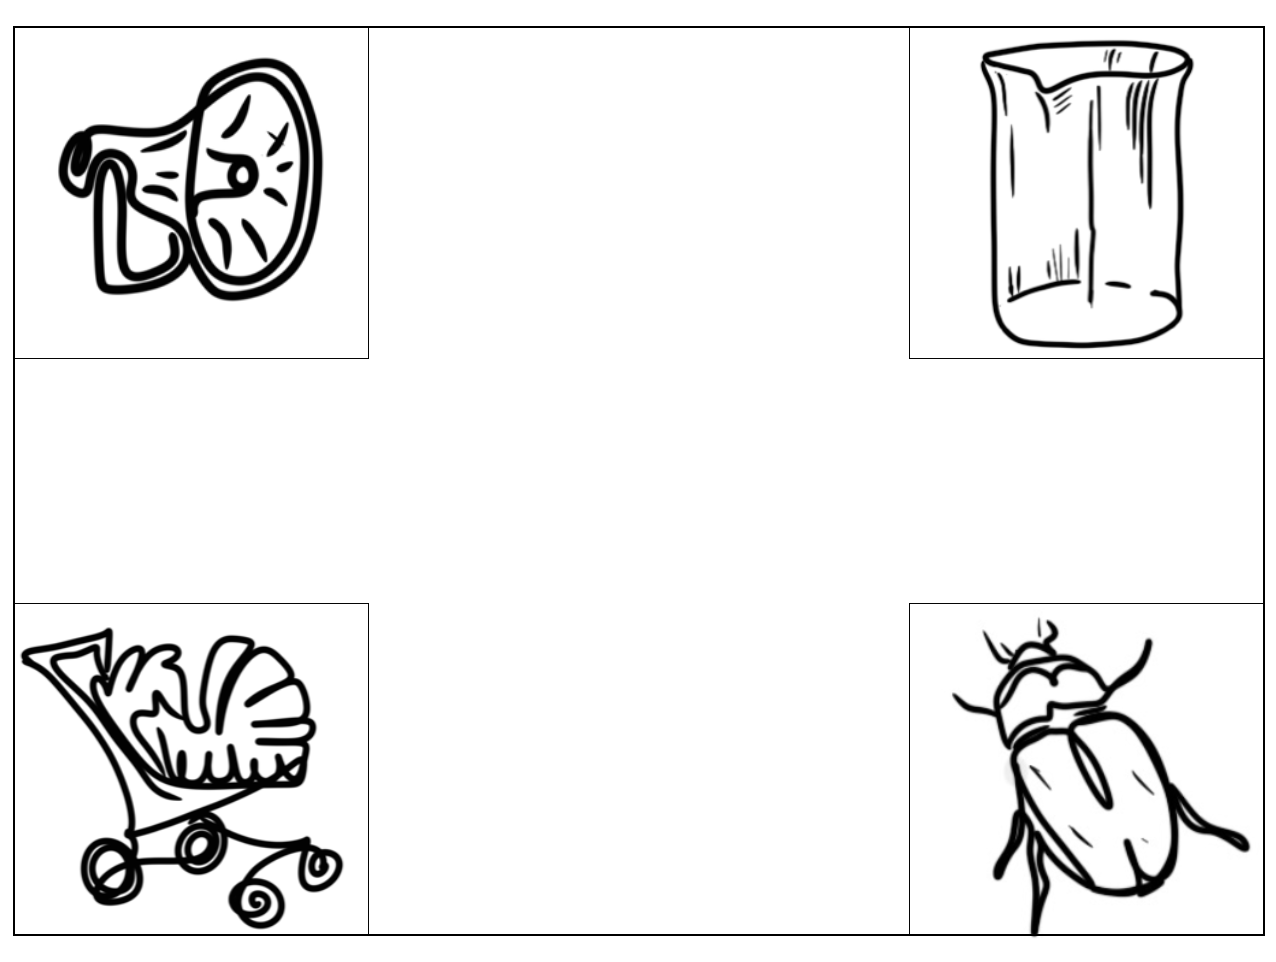
\includegraphics[scale=.35]{figures/Visual_stimuli.png}
    \caption{The four black boxes are surrounding the visual stimuli- Notice visual stimuli are maximally separated (stimuli example items are inspired by \textcite[][]{Allopenna_1998}{}{}). }
    \label{fig:Visual_stimuli.png}
\end{figure}

\textbf{Visual Stimuli.} Figure \ref{fig:Visual_stimuli.png} is an example of the visual information shown to a participant on each trial. As noted, visual stimuli can be presented simultaneously with the audio stimuli or at different points in time  \parencite{Apfelbaum_Klein-Packard_McMurray_2021}. Visual stimuli are minimally made up of two types: targets and competitors. In the case of four visual stimuli, an additional two visual stimuli include either a second competitor and a single distractor (or two distractors, if a second competitor is not built into the design). Visual stimuli are always counterbalanced across the four quadrants so as to reduce the chances of bias in eye-movements in a particular direction. Note that quadrants are absolute positions on the computer screen (e.g., upper right ('beaker' in figure \ref{fig:Visual_stimuli.png}), upper left, bottom left, bottom right). 

\textbf{Eye-Fixations.} Eye-fixations are time-stamped x- and y- coordinates on the screen that are recorded throughout a trial. In other words, where a participant is looking at a particular time. In figure \ref{fig:core_four}, red dots are specific x- and y- coordinates and red lines tie those fixations to specific times (blue dots). The rate of recording is a function of the measurements recorded per second (e.g., measuring 1000 times in one second = 1000Hz). Eye-fixations get categorized into absolute positions on the screen (quadrants) and then mapped to visual stimuli. Where a participant is looking over time is informed by the audio stimuli.

\subsection{Building an Eye-tracking Experiment in Gorilla}

Beginning with Task Builder \footnote{This section was written with both Task Builder 1 and Task Builder 2 in mind (e.g., zones and objects are the same thing). However, the terminology used will all be in Task Builder 1 style as Task Builder 2 does not yet have eye-tracking functionality.}. Each trial should start with a fixation cross for roughly 200 ms. Next, a simple forced choice task can serve as the foundation of the experiment with four visual stimuli as the choices (see Experimental ET Tasks: simple forced choice at \href{https://app.gorilla.sc/openmaterials/715241}{Gorilla link}). Audio input comes from the \gorilla{web audio} \gorilla{zone} that plays at the beginning of a specific \gorilla{screen}, whereas \gorilla{response button image} is the \gorilla{zone} for visual stimuli. The audio and visual stimuli must have a time-locked relationship. The audio stimuli will either provide suggestive hints toward a specific visual stimulus or even explicitly tell the participant which to choose. When building the experiment, it is essential to focus on the timing of the trials, the types of data you want out of the trial\footnote{Feedback is often used in multilingual studies, and would simply require an additional \gorilla{screen} indicating the correct target, such as a circle around the beaker or written corrective feedback.}, and when the webcam should track eye-fixations. 

In Gorilla, \gorilla{tasks} are made up of \gorilla{displays}, which can be thought of as trials. The \gorilla{display} is a useful unit because it allows the researcher to make recursive functionality (e.g., run the same trial with different content \textit{n} times). Within each \gorilla{display},  \gorilla{screens} are played consecutively. That is, to control the overall relationship between the timing of audio stimuli and visual stimuli (i.e., preview, simultaneous, delayed), \gorilla{web audio} should be placed either in the \gorilla{screen} before, of, or after the visual stimuli (examples for each type of timing is provided in the \href{https://app.gorilla.sc/openmaterials/715241}{Gorilla link}). As seen in figure \ref{fig:Gorilla_work_flow}, the exact location of your \gorilla{web audio} depends on where you want it time-locked to the visual stimuli in terms of \gorilla{screens}. 

\begin{figure}[h]
    \centering
    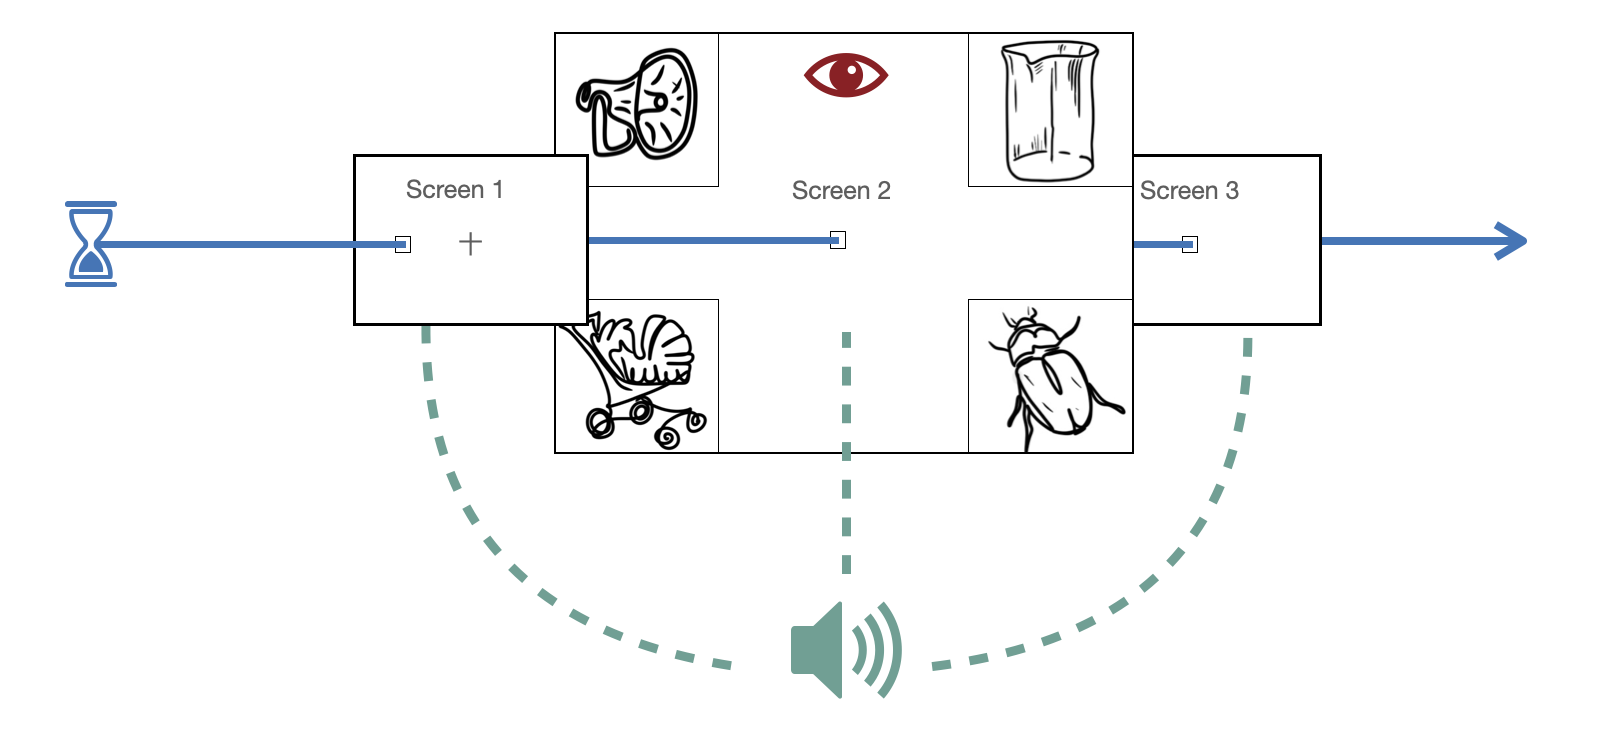
\includegraphics[scale=.5]{figures/Gorilla_work_flow.png}
    \caption{A Gorilla display example with three screens. Colors match figure \ref{fig:core_four} layout for ease.}
    \label{fig:Gorilla_work_flow}
\end{figure}

While the overall timing of a trial is controlled by the placement of \gorilla{screens}, the transition between \gorilla{screens} and fine grained timing within \gorilla{screens} is manipulated through \gorilla{zones} within each \gorilla{screen}. \gorilla{Zones} include functionality like (\gorilla{Response Buttons}, \gorilla{web audio}, and \gorilla{eye-tracker 2}). There are two general types of \gorilla{zones} which are important in the context of eye-tracking (i.e., \gorilla{content-response} and \gorilla{control}). \gorilla{Content-response} \gorilla{zones} allow the user to put in audio and visual stimuli in specific locations. Importantly, not all of the \gorilla{Content-response} \gorilla{zones} enable screen progression. For example, the \gorilla{web audio} \gorilla{zone} can end a \gorilla{screen} on completion; however, you may need the \gorilla{screen} to progress at a fixed time. In these cases, \gorilla{control} \gorilla{zones} allow a \gorilla{screen} to progress at specific time intervals between \gorilla{screens}.  

\subsection{Gorilla settings}

In each \gorilla{zone}, \gorilla{configuration settings} allow the user to enable features for both within the experiment and for data output. For example, \gorilla{screens} with \gorilla{web audio} can either progress automatically or continue until another \gorilla{zone} forces progression. Similarly, \gorilla{response button images} for the visual stimuli can end a \gorilla{screen} on-click or the \gorilla{screen} can end through control zones \gorilla{time limit section/screen}, with exact timing in \gorilla{configuration settings}. In terms of data output, each \gorilla{response-button image} should be named (e.g., image\_1) so that you can differentiate clicks in data analysis.

\gorilla{Eye-tracker 2} is found in the \gorilla{advanced zone}; it has two explicit modes: \gorilla{calibration} and \gorilla{recording}. Either a five-point or nine-point calibration can be used, with any level set for calibration fail points or repeat calibrations. Nine-point calibration provides a better standard but takes longer and may fail more often. While not fully necessary because of the manner in which webgazer.js functions \parencite[e.g.,][]{ Chen_et_al_2001}, it is recommended that the researcher calibrate participants at the beginning of the experiment and throughout the experiment \parencite[][]{Prystauka_Altmann_Rothman_2023}. We recommend always reporting calibration metrics.  

The \gorilla{recording screen} is used when the visual stimuli begins. All screens you wish to record eye-fixations for should have an \gorilla{eye-tracker zone}. The choice of \gorilla{Basic eye-tracking data} and \gorilla{detailed eye-tracking data} is in \gorilla{configuration settings}. \gorilla{Basic data} does not provide time course data, it only provides percentages of looks. For this reason, you will need to select \gorilla{detailed data}. Additionally, in cases where you want to record multiple \gorilla{screens}, you should select  \gorilla{continue recording} in \gorilla{Eye-tracker 2} \gorilla{configurations settings}. Unlike the eye-link 1000 (used in \parencite{Porretta_et_al_2020}), which measures at 1000hz, webcams have variable frame rates that depend on the lighting, participant movement, and the participant's device, which can range between 20hz and 60hz \parencite{Vos_2017}. The typical raw amount of eye-fixation samples captured per second is 15, 30, 60, and 120 (standard webcam frame rates) but likely much lower in most cases. Additionally, the lighting environment of the participant also has a strong effect on the number of fixations recorded. For example, darker rooms will lead to the camera capturing less eye-fixation per second (lower fps). This means that some trials will capture more eye-fixations than other trials \parencite{Prystauka_Altmann_Rothman_2023}. Additionally, the timing of eye-fixations can vary within a trial with non-equal measurements between captured eye fixations. On the aggregate, this means that the eye-fixations being captured start to drop throughout the trial. This variability in frame rate can be somewhat attenuated by doing in-person eye-tracking with web-gazer but is nonetheless somewhat unavoidable \parencite[e.g., ][]{Papoutsaki}. 

\subsection{Gorilla Data and Tidy Data}

Raw data from a VWP experiment downloaded from Gorilla has two basic parts: task data by \gorilla{node} and an \gorilla{uploads folder} (trial by trial specific data for each participant). This format is not limited to eye-tracking data and is true for any experiment that would need additional trial-specific data (e.g., voice recordings, mouse-tracking) beyond simple behavioral responses (e.g., reaction time, accuracy). Task data will include all selections and timings of those selections (e.g., reaction time, condition, trial order). However, the additional \gorilla{uploads folder} will contain trial by trial eye-fixation data that is paired with within-trial trial-time. A simplified example of this is shown in figure \ref{fig:data_structure}. The amount of task data sheets has a direct relationship with the number of experimental (and/or questionnaire) \gorilla{nodes} in your \gorilla{experiment}. While it depends on your design, if counterbalancing audio stimuli by conditions so that participants do not hear the same audio from two speakers, then each of these will also have their own \gorilla{node} separated by \gorilla{spreadsheets}. That is, if you were to have four counterbalanced stimuli \gorilla{spreadsheets} in your experiment design then you will have four raw task data sheets, one from each of these \gorilla{nodes} (see, Experimental ET Tasks: All, for example). However, the number of data sheets in the \gorilla{uploads folder} will depend on how many participants and trials you have. For example, if you have 60 participants who finish 48 trials, you will have a total of 2,880 eye-tracking data sheets (60X48) that reference the behavior trials in your four task data sheets. This is the size of the data we use in the data wrangling section.

\begin{figure}[ht]
    \centering
    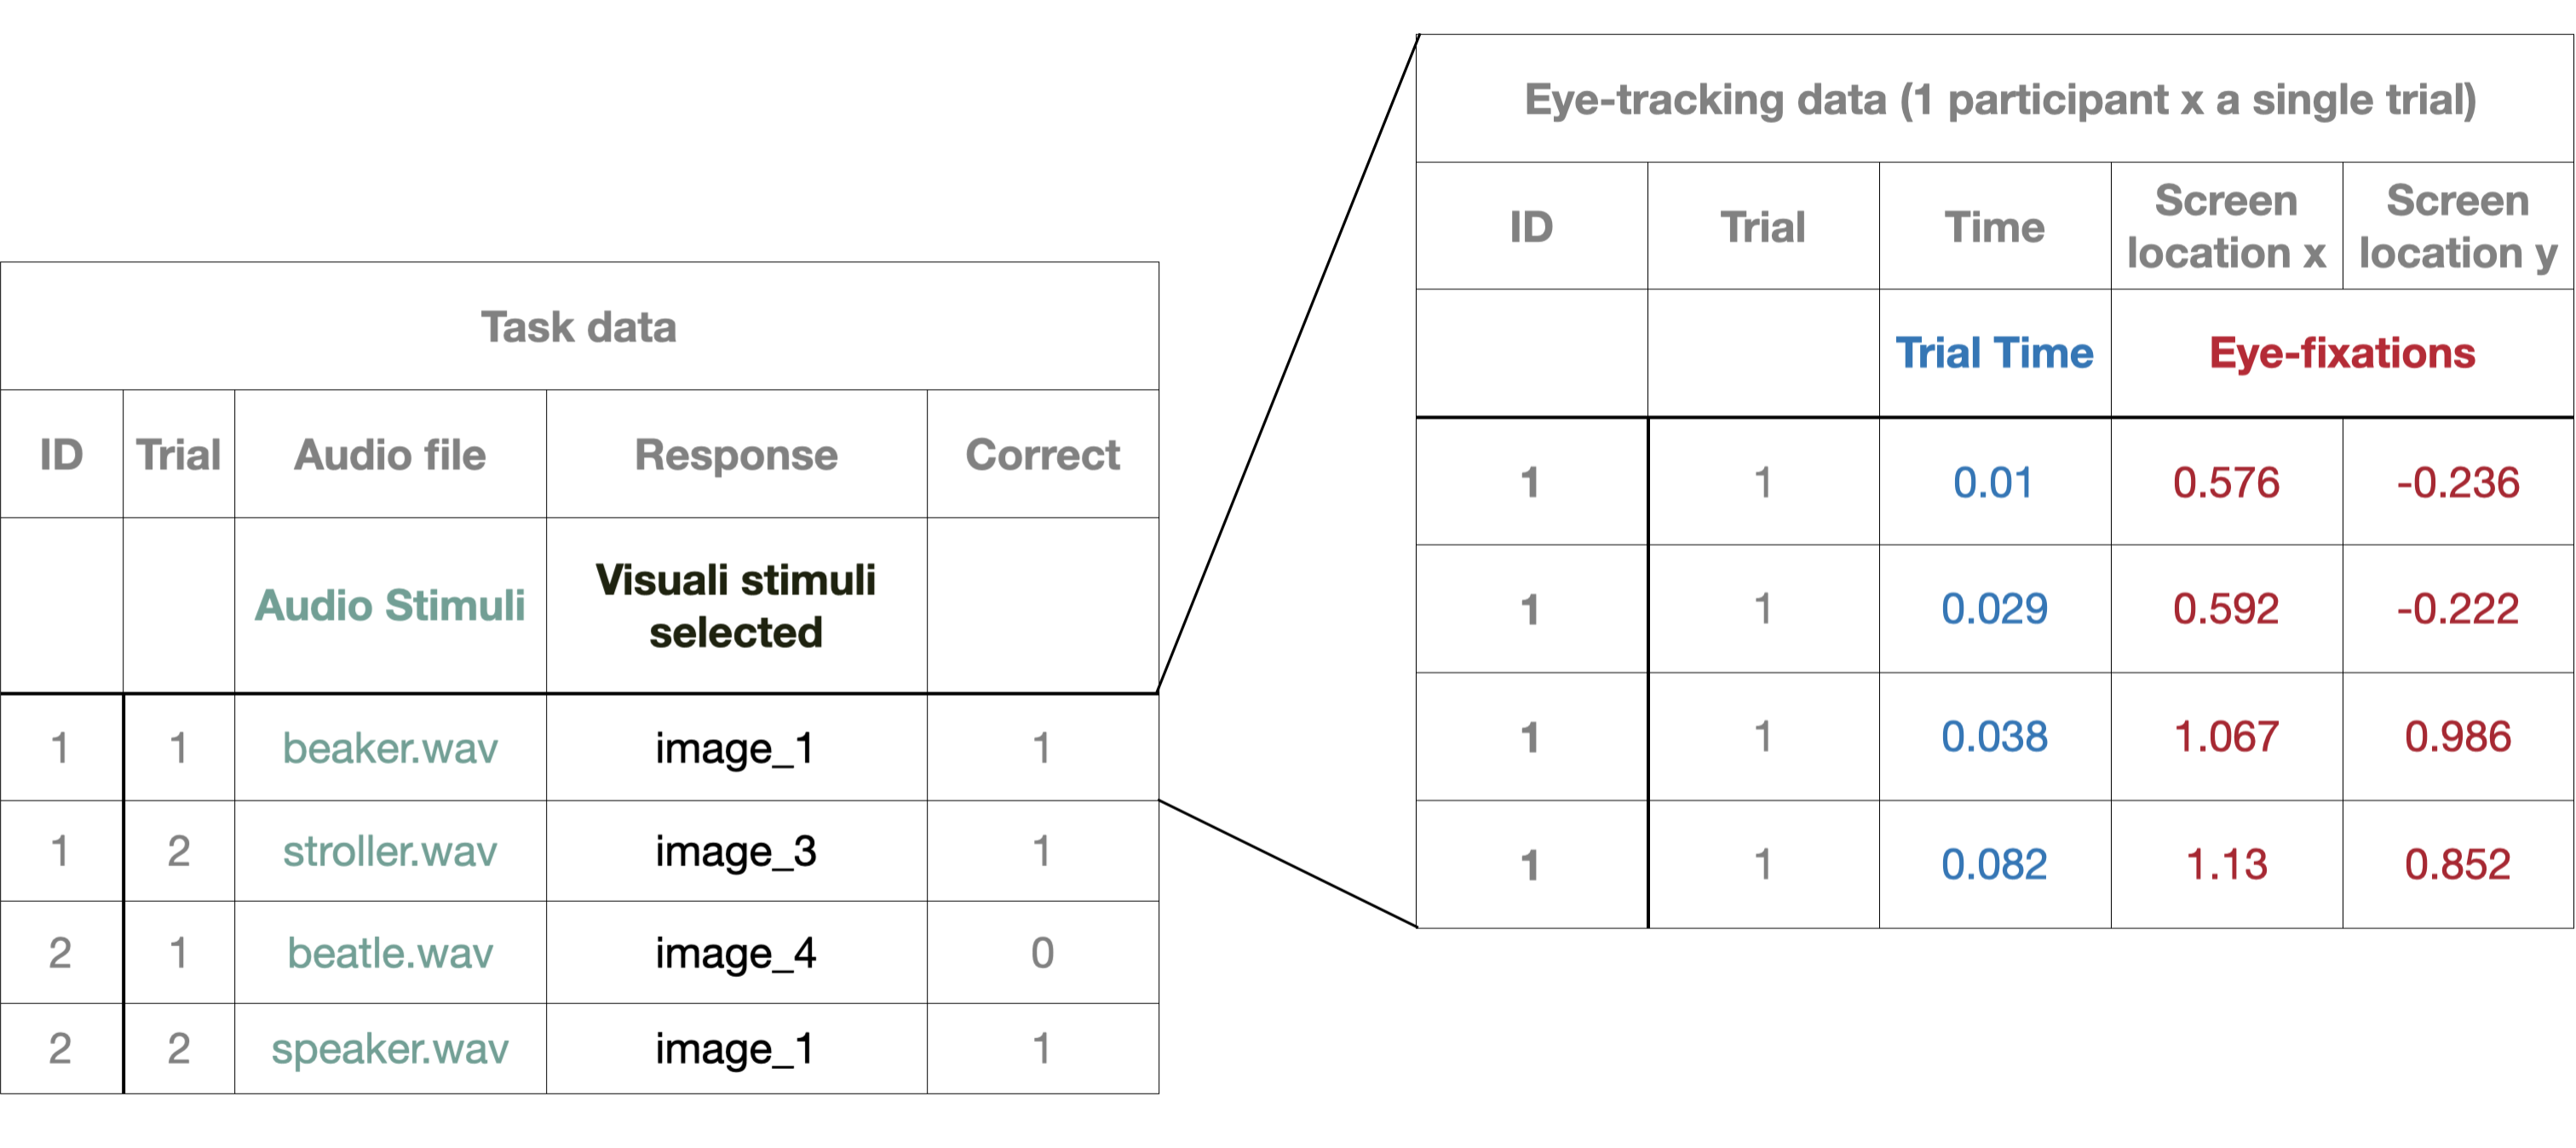
\includegraphics[scale=.3]{figures/data_structure.png}
    \caption{Task data (left) and trial by trial eye-tracking data (right)-\textit{uploads} data. Colors match figure \ref{fig:core_four} layout for ease.}
    \label{fig:data_structure}
\end{figure}

The raw data that Gorilla provides is maximally informative to enable a variety of experiments and analyses to be done. However, this also means that the data is messy. Tidy data is data where each column refers to a single variable (e.g., audio stimuli) and each row is exactly one observation (e.g., beaker.wav). However, the meaning of a single observation depends on your question. For example, if you are examining questionnaire data, it is likely that each row should have the answer to many questions, where each question is a single column. However, if you are looking at behavioral data then each row shows a different trial for each participant with their response as a single observation.


